\notepart{The one-dimensional area law}{part:arealaw}

\section{Setting, reductions, and counting}\label{sec:setting}

\begin{inwords}
To bound the entanglement entropy $S_\Om(A)$ of an arbitrary subset
$A\subseteq\Lam$ in terms of its edge boundary $\abs{\partial_\Lam A}$,
three elementary reductions allow us to restrict attention to a single
interval $X$ inside a connected chain. First, if the domain $\Lam$ has
several connected components, every interaction support has finite graph
diameter and therefore lies inside a single component; the Hamiltonian
decomposes as a sum over components, the unique ground vector factors as a
tensor product, and both the entanglement entropy and the edge boundary
are additive across components. Thus we may take $\Lam$ to be a single
interval. Second, any subset $A$ of an interval is a disjoint union of
maximal subintervals, each contributing at least one distinct boundary
edge, so subadditivity of the entropy reduces Theorem~\ref{thm:A} to the
case where $A$ is an interval. Third, an interval has at most two boundary
cut edges, and any range-$R$ interaction crossing a cut edge is supported
within a window of $2R$ consecutive sites centred at that cut. Both the
number of interactions crossing the boundary of an interval and the
logarithm of their joint Hilbert-space dimension are therefore bounded by
constants depending only on $R$ and $q$. This boundary counting is the
entire geometric input of the one-dimensional area law.
\end{inwords}

\precisely
For an interval $X\subseteq\Lam$ and a support $Y$ with
$\diam_{d_\Lam}Y\le R$, we say that $Y$ is \emph{split} by $X$ if
$Y\cap X\ne\varnothing$ and $Y\setminus X\ne\varnothing$. Since $Y$ is
contained in $R+1$ consecutive integers and contains a site on each
side of one of the two cut edges of $X$, it lies entirely in one of the
two windows of $2R$ consecutive sites centred at a cut edge. Hence
\begin{equation}\label{eq:count}
\begin{split}
 &\#\{Y:\ Y\text{ split by }X\}\le 2\cdot 2^{2R}=:N_R,\\
 &\dim\cH_Y\le q^{R+1},\qquad
 \ell_R:=\log(\e q^{R+1}).
\end{split}
\end{equation}
To separate the action of a split interaction $h_Y$ across the cut between
$X$ and $\Lam\setminus X$, we expand $h_Y$ in the matrix units $E_{ab}$ of
$\cH_{Y\cap X}$ as
\begin{equation}\label{eq:matrixunits}
 h_Y=\sum_{\alpha=1}^{N_Y}c_\alpha\otimes d_\alpha,\qquad
 N_Y\le q^{2(R+1)},\qquad \norm{c_\alpha}\,\norm{d_\alpha}\le J,
\end{equation}
with $c_\alpha$ supported in $X$ and $d_\alpha$ in $\Lam\setminus X$
(each matrix unit $E_{ab}$ on $\cH_{Y\cap X}$ has operator norm one, and
the coefficient operator $d_\alpha=\Tr_{Y\cap X}[(E_{ba}\otimes\id)h_Y]$
has norm at most $\norm{h_Y}\le J$). Put
\begin{equation}\label{eq:BR}
 \cB_R:=1+N_R\,\ell_R^2 .
\end{equation}

\begin{figure*}[t]
\centering
\begin{adjustbox}{max width=\linewidth}
\begin{tenkz}[lattice={1x14}, frame=plane, physical=up, bonds=none]
  \tn{} & \tn{} & \tn{} & \tn{} & \tn{} & \tn{} & \tn{} & \tn{} & \tn{} & \tn{} & \tn{} & \tn{} & \tn{} & \tn{}
  \tnmark[form=enclosure, species=selected, label pos=300]{(1,5) .. (1,9)}{$X$}
  \tnmark[form=bracket, species=collar, label pos=120]{(1,3) .. (1,6)}{\text{window}}
  \tnmark[form=bracket, species=collar, label pos=120]{(1,8) .. (1,11)}{\text{window}}
  \tnmark[form=enclosure, species=secondary, tint, label pos=300]{(1,8) .. (1,10)}{$Y$}
\end{tenkz}

\end{adjustbox}
\caption{An interval $X$ of the chain (drawn for $R=2$), the two windows of $2R$ sites centred on its cut edges, and two interaction supports $Y'$ and $Y$ split by $X$, one in each window. Every split support lies in a window, which is why their number is bounded by $N_R$.}\label{fig:chain-cuts}
\end{figure*}

\begin{lemma}[Reductions]\label{lem:reductions}
It suffices to prove Theorem~\ref{thm:A} for $\Lam$ an interval and $A$
an interval with $\partial_\Lam A\ne\varnothing$, with a constant
$C_{\mathrm{int}}$ bounding $S_\Om(A)$; then Theorem~\ref{thm:A} holds
with $C_{\mathrm{AL}}=C_{\mathrm{int}}$.
\end{lemma}
\begin{proof}
Let $\Lam_1,\dots,\Lam_k$ be the connected components of $\Lam$ (maximal
intervals). Every support of finite graph diameter lies in a single
component, so $H=\sum_iH_i$ with $H_i$ acting on $\cH_{\Lam_i}$. The
ground eigenspace of $H$ is the tensor product of the ground eigenspaces
of the $H_i$; since the former is one-dimensional, so is each of the
latter, hence $\Om=\bigotimes_i\Om_i$ and
$S_\Om(A)=\sum_iS_{\Om_i}(A\cap\Lam_i)$, while
$\partial_\Lam A=\bigsqcup_i\partial_{\Lam_i}(A\cap\Lam_i)$. Each $H_i$
inherits \eqref{eq:gap} with the same gap $\Delta$ (by restricting the
inequality to vectors of the form $\xi\otimes\bigotimes_{j\ne i}\Om_j$).
We may therefore assume that $\Lam$ is an interval. Write
$A=\bigsqcup_{a=1}^mA_a$ as a union of maximal subintervals. If some
$A_a=\Lam$, then $A=\Lam$ and $S(A)=0$. Otherwise each $A_a$ has at least
one boundary edge, and distinct $A_a$ have disjoint boundary edges (any
two maximal subintervals are separated by at least one site outside $A$,
so their outer cut edges are distinct). Thus $m\le\abs{\partial_\Lam A}$,
and subadditivity yields
$S(A)\le\sum_aS(A_a)\le C_{\mathrm{int}}\abs{\partial_\Lam A}$.
\end{proof}

From now on $\Lam=\{1,\dots,N\}$ and $X\subseteq\Lam$ is an interval. For
an integer $j\ge0$, write $X^{+j}=\{x\in\Lam:\dist(x,X)\le j\}$, which is
again an interval.

\section{The marginal tail bound}\label{sec:tail}

\begin{inwords}
Fix an interval $X$ and write $\Om=\sum_j\sqrt{p_j}\,u_j\otimes w_j$ for
its Schmidt decomposition across $X$ and $\Lam\setminus X$. Both the
variational filter norms in Section~\ref{sec:buffer} and the Schmidt
truncation in Part~\ref{part:mps} require controlling moments
$\Tr\rho_X^{1-u}$ of the reduced density operator in terms of the von
Neumann entropy $S(X)$ alone. Viewing the entanglement spectrum as the
probability distribution of the \emph{surprisal} $K=-\log p_j$ drawn with
probability $p_j$, whose mean is $\E K=S(X)$, this amounts to showing that
$K$ is concentrated around $S(X)$. Lemma~\ref{lem:tail} shows that the
global spectral gap forces $K$ to have sub-Gaussian moments near $u=0$ and
exponential tails around $S(X)$, with a width determined solely by $q$,
$R$, and $J/\Delta$, regardless of how large $S(X)$ may be.

The physical mechanism is a non-unitary marginal tilt. Multiply $\Om$ on
$X$ by $F=\rho_X^{-u/2}$ and renormalise: the resulting trial vector
$\Theta=F\Om/\sqrt{M(u)}$ has Schmidt probabilities $p_j^{1-u}/M(u)$, where
$M(u)=\sum_jp_j^{1-u}=\E\,\e^{uK}$ is the moment generating function of
$K$. Because $\Theta\propto F\Om$, it is an exact eigenvector of the
conjugated Hamiltonian $FHF^{-1}$ with energy $E_0$, so its excitation
energy $\langle\Theta,(H-E_0)\Theta\rangle$ equals
$\langle\Theta,(H-FHF^{-1})\Theta\rangle$. Interactions supported inside
$\Lam\setminus X$ commute with $F$ and cancel; interactions supported
inside $X$ also cancel in expectation because $F$ commutes with the tilted
marginal $\sigma=\Tr_{\Lam\setminus X}\ket\Theta\bra\Theta$. Only the at
most $N_R$ interactions split by the boundary of $X$ contribute.

To see why each split interaction $h$ contributes quadratically in $u$
rather than linearly, embed the conjugation into the analytic family
$f(z)=\langle\Theta,\sigma^{z}h\sigma^{-z}\Theta\rangle$. On the imaginary
axis $\sigma^{iy}$ is unitary, so $\abs{f(iy)}\le J$; on the strip
$\abs{\Re z}\le\frac14$, a matrix-unit expansion bounds $\abs{f(z)}$ by
$2Jq^{2(R+1)}$, and Hadamard's three-lines theorem compresses the
dimensional factor into a strip of width $\delta_R\propto\ell_R^{-1}$ on
which $\abs{f(z)}\le\e J$. Crucially, Hermiticity of $h$ gives the
reflection symmetry $f(-\bar z)=\overline{f(z)}$, which makes all odd
Taylor coefficients at the origin purely imaginary and eliminates the
linear term of $\Re(f(x)-f(0))$. Cauchy's estimate therefore bounds the
excitation energy by $O(J\cB_R u^2)$. The spectral gap converts this
quadratic energy into a quadratic lower bound on the ground-state overlap
$\abs{\langle\Om,\Theta\rangle}^2=M(u/2)^2/M(u)\ge 1-O(\vartheta\cB_R u^2)$,
or $\log M(u)\le 2\log M(u/2)+Cu^2$. Iterating this scale-halving relation
down to $u\to0$, where $\log M(u)=uS(X)+o(u)$, yields the sub-Gaussian
bound $\log M(u)\le uS(X)+Cu^2$, and Markov's inequality gives the
exponential tail bound.

In two dimensions the tail width scales as the square root of the boundary
length; in one dimension it is an $O(1)$ constant, which underpins both
parts of this note.
\end{inwords}

\precisely
Let $X\subseteq\Lam$ be an interval, let $\rho=\rho_X$ have positive
eigenvalues $p_j$, let $K$ be the random variable taking the value
$-\log p_j$ with probability $p_j$ so that $\E K=S(X)$, and put
\begin{equation}\label{eq:theta}
 \vartheta=\frac J\Delta,\qquad
 u_0=\frac{1}{32\sqrt{(1+\vartheta)\cB_R}}.
\end{equation}

\begin{lemma}[Marginal tail bound]\label{lem:tail}
For every interval $X\subseteq\Lam$ and every real $u$ with $\abs u\le u_0$,
\begin{equation}\label{eq:mgf}
 \log\Tr\rho_X^{\,1-u}=\log\E\,\e^{uK}\le u\,S(X)+512\,\e\,\vartheta\,\cB_R\,u^2 ,
\end{equation}
where $\rho_X^{1-u}$ is taken to be zero on the kernel of $\rho_X$.
Consequently, for every $w\ge0$,
\begin{equation}\label{eq:tail}
 \Pr\{\abs{K-S(X)}>w\}\le 2\e^{\e/2}\exp(-u_0w).
\end{equation}
\end{lemma}

\begin{proof}
Put $M(u)=\sum_jp_j^{1-u}$ and $L(u)=\log M(u)$; note that $L(0)=0$ and
$L'(0)=S(X)$. Let $P$ be the support projection of $\rho$, set
$F=\rho^{-u/2}$ on $P\cH_X$ and $F=\id$ on the kernel, and define
\[
 \Theta=\frac{F\Om}{\sqrt{M(u)}},\qquad
 \sigma=\Tr_{\Lam\setminus X}\ket\Theta\bra\Theta=\frac{\rho^{1-u}}{M(u)} .
\]
Since $F$ is invertible on $\cH_\Lam$, we have $FHF^{-1}\Theta=E_0\Theta$ and
\begin{equation}\label{eq:tiltenergy}
 \langle\Theta,(H-E_0)\Theta\rangle
 =\sum_Y\bigl(\langle\Theta,h_Y\Theta\rangle-\langle\Theta,Fh_YF^{-1}\Theta\rangle\bigr).
\end{equation}
A term $h_Y$ supported in $\Lam\setminus X$ commutes with $F$ and
contributes zero. A term supported in $X$ also contributes zero because
$\Tr(\sigma Fh_YF^{-1})=\Tr(\sigma h_Y)$ by $[F,\sigma]=0$ and cyclicity of
the trace. Thus only terms split by $X$ remain, and there are at most
$N_R$ of them by \eqref{eq:count}.

To bound each split term $h=h_Y$ analytic-function-theoretically, define for
$z\in\C$ the operator $\sigma^z=P\exp(z\log(\sigma|_{P\cH_X}))P$ and the
entire function $f(z)=\langle\Theta,\sigma^zh\sigma^{-z}\Theta\rangle$,
which satisfies $f(0)=\langle\Theta,h\Theta\rangle$ since $\Theta$ lies in
the support of $\sigma$. At $z_u=-u/(2(1-u))$ one has, on the support,
$\sigma^{z_u}=M(u)^{-z_u}F$ and $\sigma^{-z_u}=M(u)^{z_u}F^{-1}$, so
$f(z_u)=\langle\Theta,Fh F^{-1}\Theta\rangle$. On the imaginary axis the
powers $\sigma^{iy}$ are unitary on the support, giving $\abs{f(iy)}\le J$.
To bound $f(z)$ on the strip $\abs{\Re z}\le\tfrac14$, expand $h$ in matrix
units as in \eqref{eq:matrixunits} and write
$\Theta=\sum_j\sqrt{s_j}\,e_j\otimes f_j$ for its Schmidt decomposition
across $X$:
\[
 f(z)=\sum_\alpha\sum_{j,k}s_j^{1/2+z}s_k^{1/2-z}\,
 \langle e_j,c_\alpha e_k\rangle\langle f_j,d_\alpha f_k\rangle .
\]
For $\abs{\Re z}\le\frac14$, the weighted arithmetic--geometric mean
inequality gives $\abs{s_j^{1/2+z}s_k^{1/2-z}}\le s_j+s_k$, and for any
operators $c,d$ with matrix elements $c_{jk},d_{jk}$ the row and column
Cauchy--Schwarz inequalities yield
\begin{equation}\label{eq:rowcolumn}
 \sum_{j,k}(s_j+s_k)\,\abs{c_{jk}}\,\abs{d_{jk}}\le 2\norm c\,\norm d ,
\end{equation}
because $\sum_k\abs{c_{jk}}\abs{d_{jk}}\le\norm c\norm d$ for each row $j$ and
likewise for each column $k$, while $\sum_j s_j=1$. Hence
$\abs{f(z)}\le 2Jq^{2(R+1)}$ on $\abs{\Re z}\le\frac14$. Applying
Hadamard's three-lines theorem on each of the strips $0\le\pm\Re z\le\frac14$
gives
$\log\abs{f(x+iy)}\le\log J+4\abs x\log(2q^{2(R+1)})\le \log J+8\abs x\,\ell_R$,
so that
\begin{equation}\label{eq:narrow}
 \abs{f(z)}\le \e J\qquad\text{for }\abs{\Re z}\le\delta_R:=\frac1{8\ell_R}.
\end{equation}
Since $h=h^*$ and $(\sigma^z)^*=\sigma^{\bar z}$, we have
$f(-\bar z)=\overline{f(z)}$. In the power-series expansion
$f(z)=\sum_nc_nz^n$, the coefficient $c_n$ is therefore real for even $n$
and purely imaginary for odd $n$. For real $x$, the linear term in the
real part drops out, leaving $\Re(f(x)-f(0))=\sum_{n\ge2\text{ even}}c_nx^n$,
and Cauchy's estimate $\abs{c_n}\le\e J\delta_R^{-n}$ on the disc of
radius $\delta_R$ from \eqref{eq:narrow} gives, for $\abs x\le\delta_R/2$,
\begin{equation}\label{eq:quadratic}
 \abs{\Re(f(x)-f(0))}\le 2\e J\,x^2\delta_R^{-2}=128\,\e J\,\ell_R^2\,x^2 .
\end{equation}
For $\abs u\le u_0$ we have $\abs u\le\frac1{32}$, $\abs{z_u}\le\abs u$, and
$\ell_R\le\sqrt{\cB_R}$, so $\abs{z_u}\le\delta_R/2$. Since the left-hand
side of \eqref{eq:tiltenergy} is real, applying \eqref{eq:quadratic} at
$x=z_u$ to each of the at most $N_R$ split terms yields
\begin{equation}\label{eq:energyquad}
 0\le\langle\Theta,(H-E_0)\Theta\rangle\le 128\,\e J\,N_R\ell_R^2\,u^2
 \le 128\,\e J\,\cB_R\,u^2 .
\end{equation}
The spectral gap \eqref{eq:gap} converts this energy bound into the
overlap estimate
$1-\abs{\langle\Om,\Theta\rangle}^2\le 128\,\e\,\vartheta\,\cB_Ru^2\le\frac12$.
Since $\langle\Om,\Theta\rangle=M(u/2)/\sqrt{M(u)}$, we obtain
\[
\begin{split}
 &\frac{M(u/2)^2}{M(u)}\ge 1-128\,\e\,\vartheta\,\cB_R u^2,
 \qquad\text{i.e.}\\
 &L(u)\le 2L(u/2)+256\,\e\,\vartheta\,\cB_Ru^2,
\end{split}
\]
using $-\log(1-v)\le2v$ for $0\le v\le\frac12$. Every halving $u/2^j$
remains in $[-u_0,u_0]$, so induction over $j$ gives
\[
\begin{split}
 &L(u)\le 2^jL(u/2^j)+256\,\e\,\vartheta\,\cB_Ru^2\sum_{i<j}2^{-i}\\
 &\qquad\xrightarrow[j\to\infty]{} uS(X)+512\,\e\,\vartheta\,\cB_Ru^2 ,
\end{split}
\]
which proves \eqref{eq:mgf}. For \eqref{eq:tail}, apply Markov's inequality
to $\e^{\pm u_0(K-S(X))}$: at $u=\pm u_0$, the quadratic term in
\eqref{eq:mgf} is $512\e\vartheta\cB_R/(1024(1+\vartheta)\cB_R)\le\e/2$, so
each one-sided tail is bounded by $\e^{\e/2}\e^{-u_0w}$.
\end{proof}

\begin{figure}[t]
\centering
\begin{adjustbox}{max width=\linewidth}
\(\displaystyle \frac{1}{M(u)}\;
  \begin{tenkz}[rows={wire,wire,wire,wire}, cols=3, bonds=none]
    \tn[at=(2,1), skin=box, name=f, ports={90:physical:$X$, 270:physical}]{F}
    \tn[at=(3,1), skin=box, wide=2, name=k, ports={90@1:physical, 90@2:physical}]{\Omega}
    \tn[at=(4,1), skin=box, wide=2, name=b, ports={270@1:physical, 270@2:physical}]{\overline{\Omega}}
    \tn[at=(5,1), skin=box, name=g, ports={90:physical, 270:physical:$X$}]{\overline{F}}
    \tnwire{k.90@1}{f.270}
    \tnwire{b.270@1}{g.90}
    \tn[at=(2,2), skin=none, name=j1, ports={270:physical, 0:physical}]{}
    \tn[at=(2,3), skin=none, name=j2, ports={180:physical, 270:physical}]{}
    \tn[at=(5,3), skin=none, name=j3, ports={90:physical, 180:physical}]{}
    \tn[at=(5,2), skin=none, name=j4, ports={0:physical, 90:physical}]{}
    \tnwire{k.90@2}{j1.270} \tnwire{j1.0}{j2.180} \tnwire[name=tr]{j2.270}{j3.90}
    \tnwire{j3.180}{j4.0} \tnwire{j4.90}{b.270@2}
    \tnmark[form=label, label pos=0]{on tr 0.5}{$\Lambda\setminus X$}
  \end{tenkz}
  \;=\;
  \begin{tenkz}[cols=1]
    \tn[skin=box, ports={90:physical:$X$, 270:physical:$X$}]{\sigma}
  \end{tenkz}\)

\end{adjustbox}
\caption{The tilt as a tensor diagram. Multiplying $\Omega$ on the interval $X$ by $F=\rho_X^{-u/2}$ and tracing out the rest of the chain gives $\sigma=\rho_X^{1-u}/M(u)$. Only interactions crossing the cuts of $X$ fail to commute with $F$, so the tilted state has excitation energy of order $u^2$.}\label{fig:tilt}
\end{figure}

\begin{figure}[t]
\centering
\begin{adjustbox}{max width=\linewidth}
\begin{tikzpicture}[x=1cm, y=1cm, line width=0.3pt,
    lab/.style={font=\small, inner sep=1pt},
    name/.style={font=\scriptsize, text=black!55, inner sep=1pt},
    brace/.style={decorate, decoration={brace, mirror, amplitude=3pt}},
    cut/.style={dashed, color=orange!80!black, line width=0.5pt}]
  \def\S{3.4}\def\w{1.8}\def\decay{1}\def\xmax{9.6}\def\xmin{-0.4}
  \fill[orange!30] plot[domain=5.2:\xmax, samples=60, smooth]
    (\x, {2/cosh(\x-\S)}) -- (\xmax, 0) -- (5.2, 0) -- cycle;
  \draw[black!55] (\xmin, 0) -- (\xmax, 0);
  \draw[black!55] (\xmin, 0) -- (\xmin, 2.2);
  \node[lab, anchor=north east] at (\xmax, -0.05) {surprisal \(K=-\log p\)};
  \node[lab, anchor=south, rotate=90] at (\xmin-0.18, 1.1) {probability};
  \draw[blue!65!black, line width=0.6pt] plot[domain=\xmin:\xmax, samples=120, smooth]
    (\x, {2/cosh(\x-\S)});
  \node[name, anchor=south west] at (\S+0.12, 2.0) {mean \(S(X)\)};
  \draw[black!55] (\S, 0.06) -- (\S, -0.06);
  \node[lab, anchor=north] at (\S, -0.08) {\(S(X)\)};
  \draw[cut] (\S-\w, 0) -- (\S-\w, 1.3);
  \draw[cut] (\S+\w, 0) -- (\S+\w, 1.3);
  \node[lab, anchor=north, text=orange!80!black] at (\S-\w, -0.08) {\(S(X)-w\)};
  \node[lab, anchor=north, text=orange!80!black] at (\S+\w, -0.08) {\(S(X)+w\)};
  \draw[black!55, {Bar}-{Bar}, line width=0.4pt] (\S+\w, 0.85) -- (\S+\w+\decay, 0.85);
  \node[lab, anchor=south] at (\S+\w+0.5*\decay, 0.88) {\(1/u_0\)};
  \node[name, anchor=west] at (\S+\w+\decay+0.1, 0.85) {depends only on \(q\), \(R\), \(J/\Delta\)};
  \node[lab, anchor=west, text=orange!80!black] at (\S+\w+1.7, 0.42)
    {mass \(\le 2\mathrm{e}^{\mathrm{e}/2}\mathrm{e}^{-u_0w}\)};
  \draw[orange!80!black, -{Stealth[length=3pt]}] (\S+\w+1.65, 0.38) -- (\S+\w+1.1, 0.12);
  \draw[brace, black!55] (\xmin, -0.42) -- (\S+\w, -0.42)
    node[lab, midway, below=4pt] {at most \(\mathrm{e}^{S(X)+w}\) eigenvalues with \(K\le S(X)+w\)}
    node[name, midway, below=16pt] {kept by the truncation};
\end{tikzpicture}

\end{adjustbox}
\caption{Schematic law of the surprisal. The tails decay exponentially at rate $u_0$; the mass beyond $S(X)+w$ is at most $2e^{e/2}e^{-u_0w}$, and at most $e^{S(X)+w}$ eigenvalues lie to the left of that line. Both facts are reused for the sequential truncation in Part II.}\label{fig:tail-sketch}
\end{figure}

\begin{remark}[Rényi entropies near one]\label{rem:renyi}
For $0<u\le u_0$ and $\alpha=1-u$, \eqref{eq:mgf} reads
$S_\alpha(X)=\frac{1}{u}\log\Tr\rho_X^{\alpha}\le S(X)+512\e\vartheta\cB_R(1-\alpha)$.
Since $S_\alpha\ge S$ for $\alpha<1$, all Rényi entropies of order
$\alpha\in[1-u_0,1]$ of an interval lie within $16\e\sqrt{(1+\vartheta)\cB_R}$ of its von
Neumann entropy. This is used in Section~\ref{sec:shortcut}.
\end{remark}

\section{The buffered discount with a constant-width buffer}\label{sec:buffer}

\begin{inwords}
This section establishes the core variational estimate of Part~\ref{part:arealaw}.
Conditioning an interval $X$ on a buffer $T$ of a constant number of
nearby sites halves its entropy, up to an additive constant:
\[
 S(X\,|\,T)\ \le\ \tfrac12\,S(X)+C .
\]
To keep the excitation energy of the filtered vector below the gap
$\Delta$, the filtering is distributed across $m$ concentric shells
$X_j=X^{+jD}$ ($j=1,\dots,m$), each wider than the previous one by a step $D=R$, with flanking buffers
$T_j=X_j\setminus X$ and small per-shell weight $a_j=2/m$ summing to
$\sum_j a_j=2$. Choosing $m$ of order $1+J/\Delta$ keeps the total buffer
$T=T_m$ of \emph{constant} width $mD$ on each side of $X$.

Specifically, we apply to $\Om$ a product $K=L_m\cdots L_1$ of positive
operators $L_j$ acting on $X_j$, each normalised by $\Tr L_j^{2/a_j}=1$,
and maximise the norm $N=\norm{K\Om}$. Two complementary bounds on the
maximum $N$ yield the discount.

\emph{Upper bound on $N$ (lower bound on $-2\log N$).} Computing the
excitation energy of the normalised filtered vector $\phi=K\Om/N$ requires
controlling the conjugation of each Hamiltonian term by all $m$ filters.
At a maximiser of $N$, however, unitary stationarity implies that each
filter $L_j$ commutes with the reduced density operator $\rho_j$ of $\phi$
on its own shell $X_j$. This commutation gives a \emph{stripping
identity}: any operator supported inside $X_k$ is unchanged in expectation
when conjugated by the outer filter $L_k$. Because consecutive shells are
separated by $D\ge R$, any range-$R$ interaction $h_Y$ is split by at most
one shell $X_j$; all outer filters ($k>j$) contain $Y$ and strip away,
while all inner filters ($k<j$) are disjoint from $Y$ and commute past
$h_Y$. Thus $h_Y$ is conjugated by $L_j$ alone. Diagonal stationarity clips
the log-eigenvalue differences of $L_j$ to $a_j/2$ times those of $\rho_j$,
so conjugation by $L_j$ changes the expectation of $h_Y$ by at most
$O(Ja_j^2)$. Summing over the $m$ shells and the at most $N_R$ interactions
split by each shell bounds the excitation energy of $\phi$ by
$O(J\sum_j a_j^2)=O(J/m)$. The spectral gap then ensures a ground-state
overlap $\abs{\langle\Om,\phi\rangle}^2\ge 1-C/(m\Delta)$, and the same
holds for every prefix optimiser. Using this overlap to peel the filters
$L_j$ off one at a time, and bounding each peeled factor by
$\norm{L_j\Om}\le\exp(-a_jS(X_j)/2+Ca_j^2)$ via Schatten--Hölder and the
marginal tail bound (Lemma~\ref{lem:tail}), gives
$-2\log N\ge\sum_ja_jS(X_j)-C$.

\emph{Lower bound on $N$ (upper bound on $-2\log N$).} Conversely, we test
the variational maximum on trial filters that ``pin'' a single Schmidt
vector $u_i$ of $\Om=\sum_i\sqrt{p_i}\,u_i\otimes w_i$ across $X$: namely
$L_j=\ket{u_i}\bra{u_i}\otimes M_j$, where $M_j$ acts only on the flank
$T_j$. This decouples $X$ and produces $\sqrt{p_i}\,u_i$ tensored with
$M_m\cdots M_1w_i$. Because the flank filters $M_j$ act on nested sets and
need not commute, we relate the norm of their product to the sum of single-flank
entropies via three-lines interpolation on $M_m^z\cdots M_1^zw_i$, finding
that $M_j$ can be chosen so that
$\norm{M_m\cdots M_1w_i}\ge\exp(-\sum_ja_jS_{w_i}(T_j)/2)$. Averaging over
$i$ with weights $p_i$ and applying concavity of the entropy gives
$-2\log N\le S(X)+\sum_ja_jS(T_j)$.

Subtracting the two bounds yields $\sum_ja_j\,[S(X_j)-S(T_j)]\le S(X)+C$.
Here $S(X_j)-S(T_j)=S(X|T_j)$, which is monotone decreasing in $j$ by
strong subadditivity. Since $\sum_ja_j=2$, the discount follows. No
property of the state on the flanks is used beyond their containing a
constant number of sites, and no spectral gap of any restricted
Hamiltonian is invoked.
\end{inwords}

\precisely
Fix $D=R$ (recall $R\ge1$) and an integer $m\ge4$. For an interval $X\subseteq\Lam$
put
\[
\begin{split}
 &X_0=X,\qquad X_j=X^{+jD}\ (1\le j\le m),\\
 &T_j=X_j\setminus X,
 \qquad a_j=\frac2m .
\end{split}
\]
Then $T_1\subseteq\cdots\subseteq T_m$, each $T_j$ consists of at most two
intervals of length at most $jD$, and $\sum_ja_j=2$. Define the constants
\begin{equation}\label{eq:CE}
\begin{split}
 &C_E:=8\,N_R\,J\,q^{2(R+1)},\\
 &m:=\Bigl\lceil\max\Bigl\{4,\ \frac{4C_E}{\Delta},\ 128\sqrt{(1+\vartheta)\cB_R},\\
 &\qquad\qquad\qquad
 4096\,\e\,(1+\vartheta)\,\cB_R\Bigr\}\Bigr\rceil .
\end{split}
\end{equation}
Every entry in the maximum is bounded by a function of $q,R$ times
$(1+J/\Delta)$, so
\begin{equation}\label{eq:mbound}
 m\le C_1(q,R)\,(1+\vartheta).
\end{equation}

\begin{figure*}[t]
\centering
\begin{adjustbox}{max width=\linewidth}
\begin{tenkz}[lattice={1x14}, frame=plane, physical=up, bonds=none]
  \tn{} & \tn{} & \tn{} & \tn{} & \tn{} & \tn{} & \tn{} & \tn{} & \tn{} & \tn{} & \tn{} & \tn{} & \tn{} & \tn{}
  \tnmark[form=enclosure, species=selected, label pos=s]{(1,6) .. (1,8)}{$X$}
  \tnmark[form=enclosure, species=secondary, label pos=n]{(1,4) .. (1,10)}{$X_1=X^{+D}$}
  \tnmark[form=enclosure, species=collar, label pos=150]{(1,2) .. (1,12)}{$X_2=X^{+2D}$}
  \tnmark[form=bracket, species=complement, label pos=s]{(1,4) .. (1,5)}{$T_1$}
  \tnmark[form=bracket, species=complement, label pos=s]{(1,9) .. (1,10)}{$T_1$}
  \tnmark[form=bracket, species=complement, label pos=s]{(1,2) .. (1,5)}{$T_2$}
  \tnmark[form=bracket, species=complement, label pos=s]{(1,9) .. (1,12)}{$T_2$}
\end{tenkz}

\end{adjustbox}
\caption{The interval $X$ and the nested shells $X_1=X^{+D}\subset X_2=X^{+2D}$, drawn with $D=R=2$; the braces mark the flanks $T_j=X_j\setminus X$, each a union of at most two intervals of length at most $jD$, which carry the buffer.}\label{fig:chain-shells}
\end{figure*}

\begin{lemma}[Single splitting]\label{lem:singlesplit}
A support $Y$ with $\diam_{d_\Lam}Y\le R$ is split by at most one of the
intervals $X_1,\dots,X_m$. If it is split by $X_j$, it is contained in
$X_i$ for every $i>j$ and disjoint from $X_i$ for every $i<j$. The same
holds verbatim for the family $X_0,\dots,X_m$.
\end{lemma}
\begin{proof}
Suppose $Y$ is split by $X_j$. Then $Y$ contains a site $y\notin X_j$ and
a site $x\in X_j$, and all sites of $Y$ lie within graph distance $R\le D$
of both $x$ and $y$. Every site within distance $D$ of $X_j$ belongs to
$X_{j+1}$, so $Y\subseteq X_{j+1}\subseteq X_i$ for all $i>j$. Conversely,
every site of $X_{j-1}$ lies at distance greater than $D$ from $\Lam\setminus X_j$
(since $X_j=X_{j-1}^{+D}$), so $Y\cap X_{j-1}=\varnothing$, and hence
$Y\cap X_i=\varnothing$ for all $i<j$. A set that is contained in $X_i$ or
disjoint from $X_i$ is not split by $X_i$.
\end{proof}

\begin{lemma}[Buffered discount]\label{lem:buffer}
With $m$ as in \eqref{eq:CE}, every interval $X\subseteq\Lam$ satisfies
\begin{equation}\label{eq:discount}
 S(X\,|\,T_m)\ \le\ \frac12\,S(X)+\frac12+\frac{C_E}{\Delta}.
\end{equation}
\end{lemma}

\begin{proof}
If $X=\varnothing$ both sides vanish. Assume $X\ne\varnothing$.

\paragraph{The optimisation.}
To ensure that the feasible sets are nonempty and every filter is invertible,
fix $\epsilon>0$ so small that $(\dim\cH_{X_j})\epsilon^{2/a_j}<1$ for all
$j$, and maximise
\[
 N=\norm{L_m\cdots L_1\Om}
\]
over positive operators $L_j$ on $\cH_{X_j}$ (extended by the identity on
$\Lam\setminus X_j$) satisfying $L_j\ge\epsilon\id$ and
$\Tr_{\cH_{X_j}}L_j^{2/a_j}=1$. The feasible sets are nonempty and compact
and every feasible product is invertible, so a maximum $N>0$ is attained.
At a maximiser put $K=L_m\cdots L_1$, $\phi=K\Om/N$, and
$\rho_j=\Tr_{\Lam\setminus X_j}\ket\phi\bra\phi$.

\begin{figure*}[t]
\centering
\begin{adjustbox}{max width=\linewidth}
\(\displaystyle N=\Biggl\|
  \begin{tenkz}[rows={wire,wire,wire,wire}, cols=7, bonds=none]
    \tn[at=(4,1), skin=box, wide=7, name=o,
        ports={90@1:physical, 90@2:physical, 90@3:physical, 90@4:physical,
               90@5:physical, 90@6:physical, 90@7:physical}]{\Omega}
    \tn[at=(3,3), skin=box, wide=3, name=l1,
        ports={270@1:physical, 270@2:physical, 270@3:physical,
               90@1:physical, 90@2:physical, 90@3:physical}]{L_1}
    \tn[at=(2,2), skin=box, wide=5, name=l2,
        ports={270@1:physical, 270@2:physical, 270@3:physical, 270@4:physical, 270@5:physical,
               90@1:physical, 90@2:physical, 90@3:physical, 90@4:physical, 90@5:physical}]{L_2}
    \tn[at=(1,1), skin=box, wide=7, name=l3,
        ports={270@1:physical, 270@2:physical, 270@3:physical, 270@4:physical,
               270@5:physical, 270@6:physical, 270@7:physical,
               90@1:physical:$T_3$, 90@2:physical, 90@3:physical, 90@4:physical:$X$,
               90@5:physical, 90@6:physical, 90@7:physical:$T_3$}]{L_3}
    \tnwire{o.90@3}{l1.270@1} \tnwire{o.90@4}{l1.270@2} \tnwire{o.90@5}{l1.270@3}
    \tnwire{l1.90@1}{l2.270@2} \tnwire{l1.90@2}{l2.270@3} \tnwire{l1.90@3}{l2.270@4}
    \tnwire{o.90@2}{l2.270@1} \tnwire{o.90@6}{l2.270@5}
    \tnwire{l2.90@1}{l3.270@2} \tnwire{l2.90@2}{l3.270@3} \tnwire{l2.90@3}{l3.270@4}
    \tnwire{l2.90@4}{l3.270@5} \tnwire{l2.90@5}{l3.270@6}
    \tnwire{o.90@1}{l3.270@1} \tnwire{o.90@7}{l3.270@7}
  \end{tenkz}
  \Biggr\|\)

\end{adjustbox}
\caption{The optimized norm. Three positive filters $L_1,L_2,L_3$ act on the nested intervals $X_1\subset X_2\subset X_3$ of the ground vector; each is normalized by $\mathrm{Tr}\,L_j^{2/a_j}=1$.}\label{fig:filter-product}
\end{figure*}

\paragraph{Stationarity.}
To eliminate outer filters when evaluating expectations of operators
supported in inner shells, we prove that $[L_j,\rho_j]=0$ for all $j$ by
descending induction on $j$. The key mechanism is the stripping identity:
if $[L_k,\rho_k]=0$ and $T$ is supported in $X_k$, then
\begin{equation}\label{eq:strip}
 \langle\phi,L_kTL_k^{-1}\phi\rangle=\Tr(L_k^{-1}\rho_kL_kT)=\Tr(\rho_kT)=\langle\phi,T\phi\rangle .
\end{equation}
Assume $[L_k,\rho_k]=0$ for all $k>j$ and let $B$ be anti-Hermitian on
$\cH_{X_j}$. Replacing $L_j$ by $\e^{tB}L_j\e^{-tB}$ preserves both
constraints, so the derivative of $\log\norm{K\Om}$ at $t=0$ vanishes.
That derivative equals
$\Re\langle\phi,K_{>j}(B-L_jBL_j^{-1})K_{>j}^{-1}\phi\rangle$ with
$K_{>j}=L_m\cdots L_{j+1}$. Because $B-L_jBL_j^{-1}$ is supported in
$X_j\subseteq X_{j+1}\subseteq\cdots\subseteq X_m$, we can strip $L_m$ by
\eqref{eq:strip}, then $L_{m-1}$, and so on down to $L_{j+1}$. Since
$\Tr(\rho_jB)$ is purely imaginary, stationarity yields
$\Re\Tr(L_j^{-1}\rho_jL_jB)=0$ for all anti-Hermitian $B$. Hence
$L_j^{-1}\rho_jL_j$ is Hermitian, i.e.\ equal to $L_j\rho_jL_j^{-1}$, so
$\rho_j$ commutes with $L_j^2$ and therefore with $L_j\ge0$. No
commutation between distinct filters is claimed or used.

To bound the eigenvalue ratios of $L_j$ in terms of those of $\rho_j$,
choose a common eigenbasis of $L_j$ and $\rho_j$ with eigenvalues $l_i$
and $p_i$, and set $x_i=l_i^{2/a_j}$, so that $\sum_ix_i=1$ and
$x_i\ge\epsilon^{2/a_j}$. A diagonal variation of $L_j$ together with the
same stripping of $K_{>j}$ gives
$d\log N=\frac{a_j}2\sum_ip_i\,dx_i/x_i$. By the Kuhn--Tucker conditions
on the simplex with floor $\epsilon^{2/a_j}$, the ratio $p_i/x_i$ equals a
constant $\lambda>0$ on all coordinates above the floor and is at most
$\lambda$ on floored coordinates (at least one coordinate lies strictly
above the floor by the choice of $\epsilon$, and $\lambda>0$ because
shifting weight from a zero-probability free coordinate to a
positive-probability floored coordinate would strictly increase $N$). Thus
$x_i=\max\{\epsilon^{2/a_j},p_i/\lambda\}$. Because taking a maximum with
a common floor contracts differences of logarithms, we obtain
\begin{equation}\label{eq:clip}
 \Bigl|\log\frac{l_i}{l_k}\Bigr|\le\frac{a_j}{2}\Bigl|\log\frac{p_i}{p_k}\Bigr|
 \qquad(p_i,p_k>0).
\end{equation}

\paragraph{Energy of the optimised vector.}
Since $KHK^{-1}\phi=E_0\phi$, the excitation energy of $\phi$ is
\[
 \langle\phi,(H-E_0)\phi\rangle=\sum_Y\Re\bigl(\langle\phi,h_Y\phi\rangle-\langle\phi,Kh_YK^{-1}\phi\rangle\bigr).
\]
If $Y$ is split by none of $X_1,\dots,X_m$, then by
Lemma~\ref{lem:singlesplit} each $X_j$ either contains $Y$ or is disjoint
from $Y$; stripping the containing filters from the outside in via
\eqref{eq:strip} and commuting the disjoint filters past $h_Y$ shows that
the summand vanishes. If $Y$ is split by $X_j$, the same reduction strips
$L_m,\dots,L_{j+1}$ and commutes $L_{j-1},\dots,L_1$ past $h_Y$, leaving
only the single-filter difference
$\langle\phi,h_Y\phi\rangle-\langle\phi,L_jh_YL_j^{-1}\phi\rangle$. Write
$\phi=\sum_i\sqrt{p_i}\,e_i\otimes f_i$ for the Schmidt decomposition of
$\phi$ across $X_j$, where the $e_i$ are chosen in a common eigenbasis of
$\rho_j$ and $L_j$ (diagonalising $L_j$ within each eigenspace of
$\rho_j$), and put
$h_{ik}=\langle e_i\otimes f_i,h_Y(e_k\otimes f_k)\rangle$. Pairing
$(i,k)$ with $(k,i)$ and using $h_{ki}=\overline{h_{ik}}$ gives
\[
\begin{split}
 &\Re\langle\phi,L_jh_YL_j^{-1}\phi\rangle-\langle\phi,h_Y\phi\rangle\\
 &\qquad=\sum_{i,k:\,p_ip_k>0}\sqrt{p_ip_k}\,\bigl(\cosh(\log(l_i/l_k))-1\bigr)\Re h_{ik}.
\end{split}
\]
Set $z=\frac12\log(p_i/p_k)$. By \eqref{eq:clip} and $a_j\le\frac12$, we
have
$\cosh(\log(l_i/l_k))-1\le\cosh(a_jz)-1\le\frac12a_j^2z^2\cosh(a_jz)\le\frac12a_j^2z^2\cosh(z/2)$,
while $\sqrt{p_ip_k}=(p_i+p_k)/(2\cosh z)$. Since
$\sup_z z^2\cosh(z/2)/(4\cosh z)\le1$, the prefactor of $\Re h_{ik}$ is at
most $a_j^2(p_i+p_k)$. Expanding $h_Y$ in matrix units via
\eqref{eq:matrixunits} and applying \eqref{eq:rowcolumn} to each product
term yields
\[
 \bigl|\Re\langle\phi,L_jh_YL_j^{-1}\phi\rangle-\langle\phi,h_Y\phi\rangle\bigr|
 \le 2a_j^2\,q^{2(R+1)}J .
\]
Summing over $j=1,\dots,m$ and the at most $N_R$ interactions split by
each $X_j$ gives
\begin{equation}\label{eq:energy}
\begin{split}
 &0\le\langle\phi,(H-E_0)\phi\rangle\le\sum_{j=1}^m N_R\cdot 2a_j^2q^{2(R+1)}J\\
 &\qquad=\frac{8N_RJq^{2(R+1)}}{m}=\frac{C_E}{m}.
\end{split}
\end{equation}
By the spectral gap \eqref{eq:gap} and the definition of $m$ in \eqref{eq:CE},
\begin{equation}\label{eq:overlap}
 1-\abs{\langle\Om,\phi\rangle}^2\le\frac{C_E}{m\Delta}\le\frac14 .
\end{equation}
The exact same bound holds for the optimiser of every prefix
$L_j\cdots L_1$ ($1\le j\le m$): the stationarity and energy arguments
apply verbatim to the $j$-shell problem with the same weights and floor,
and any interaction split by $X_k$ with $k>j$ is disjoint from
$X_1,\dots,X_j$ and contributes zero, so the prefix excitation energy is
bounded by the sum in \eqref{eq:energy} truncated to $i\le j$.

\begin{figure*}[t]
\centering
\begin{adjustbox}{max width=\linewidth}
\(\displaystyle \begin{gathered}
    \langle\phi,Kh_YK^{-1}\phi\rangle
    \;=\;
    \Bigl\langle\phi,\;
    \begin{quantikz}
      \lstick{$X_{j-1}$} & \gate[2]{L_j^{-1}} & & \gate[2]{L_j} & \\
      \lstick{$X_j\setminus X_{j-1}$} & & \gate[2]{h_Y} & & \\
      \lstick{$\Lambda\setminus X_j$} & & & &
    \end{quantikz}
    \;\phi\Bigr\rangle
    \\[2pt]
    \text{\small outer filters $L_{j+1},\dots,L_m$: stripped by the stripping identity, $[L_k,\rho_k]=0$}
    \\[-1pt]
    \text{\small inner filters $L_1,\dots,L_{j-1}$: disjoint from $Y$, commute with $h_Y$}
  \end{gathered}\)

\end{adjustbox}
\caption{Why the energy is small. An interaction $h_Y$ split by $X_j$ is conjugated by exactly one filter: the outer filters, whose regions contain $Y$, are stripped by the stripping identity at the optimum, and the inner ones commute with $h_Y$ because they live on disjoint sites.}\label{fig:qc-single-split}
\end{figure*}

\paragraph{Upper bound on the optimum.}
To peel the filters off one by one, let $N_j$ be the maximum norm for the
prefix $1,\dots,j$ at the same floor $\epsilon$ (with $N_0=1$), and let
$L_j\cdots L_1$ be a prefix-$j$ maximiser with $K_{<j}=L_{j-1}\cdots L_1$.
Applying \eqref{eq:overlap} to the prefix-$j$ maximiser and using
Cauchy--Schwarz gives
\[
\begin{split}
 &\sqrt{1-C_E/(m\Delta)}\;N_j\le\abs{\langle\Om,L_jK_{<j}\Om\rangle}\\
 &\qquad=\abs{\langle L_j\Om,K_{<j}\Om\rangle}\le\norm{L_j\Om}\,N_{j-1}.
\end{split}
\]
For any feasible $L_j$, Schatten--Hölder with conjugate exponents
$\frac1{1-a_j}$ and $\frac1{a_j}$ together with $\Tr L_j^{2/a_j}=1$ gives
\[
 \norm{L_j\Om}^2=\Tr\rho_{X_j}L_j^2\le\bigl(\Tr\rho_{X_j}^{1/(1-a_j)}\bigr)^{1-a_j}.
\]
Applying Lemma~\ref{lem:tail} to the interval $X_j$ at
$u=-a_j/(1-a_j)$ (which satisfies $\abs u\le 2a_j=4/m\le u_0$ by
\eqref{eq:CE}) and using $(1-a_j)u^2\le 2a_j^2$ yields
\[
 \log\norm{L_j\Om}^2\le -a_jS(X_j)+1024\,\e\,\vartheta\,\cB_R\,a_j^2 .
\]
Multiplying the recursion $N_j\le(1-C_E/(m\Delta))^{-1/2}\norm{L_j\Om}N_{j-1}$
over $j=1,\dots,m$ and using $-\frac12\log(1-v)\le v$ for $0\le v\le\frac12$,
we obtain
\[
\begin{split}
 &\log N\le-\frac12\sum_ja_jS(X_j)+512\,\e\,\vartheta\,\cB_R\sum_ja_j^2+\frac{mC_E}{m\Delta}\\
 &\qquad\le -\frac12\sum_ja_jS(X_j)+\frac12+\frac{C_E}{\Delta},
\end{split}
\]
since $\sum_ja_j^2=4/m\le 1/(1024\e\vartheta\cB_R)$ by \eqref{eq:CE}. Equivalently,
\begin{equation}\label{eq:lowerN}
 -2\log N\ \ge\ \sum_{j=1}^ma_jS(X_j)-1-\frac{2C_E}{\Delta},
\end{equation}
with constants independent of the floor $\epsilon$.

\paragraph{Lower bound on the optimum by Schmidt pinning.}
Letting $\epsilon\downarrow0$, the floored maxima converge to the supremum
$N$ over all nonnegative filters $L_j\ge0$ satisfying $\Tr L_j^{2/a_j}=1$
(since the feasible sets are compact and every nonnegative feasible filter
is a limit of strictly positive feasible ones), and \eqref{eq:lowerN}
continues to hold. Write $\Om=\sum_i\sqrt{p_i}\,u_i\otimes w_i$ ($p_i>0$)
for the Schmidt decomposition across $X$. For each fixed $i$, test $N$ on
the trial filters
\[
\begin{split}
 &L_j=\ket{u_i}\bra{u_i}\otimes M_j,\qquad M_j\ge0\text{ on }\cH_{T_j},\\
 &\Tr M_j^{2/a_j}=1,
\end{split}
\]
which are feasible (since $\Tr_{X_j}L_j^{2/a_j}=\Tr M_j^{2/a_j}=1$) and give
$N\ge\sqrt{p_i}\,N_i$, where $N_i=\sup\norm{M_m\cdots M_1w_i}$ over such $M_j$.
We claim that
\begin{equation}\label{eq:trial}
 \log N_i\ge-\frac12\sum_ja_jS_{w_i}(T_j).
\end{equation}
Because the flank filters $M_1,\dots,M_m$ act on nested regions
$T_1\subseteq\cdots\subseteq T_m$ and need not commute, we relate the
product norm $N_i$ to single-flank expectations by complex interpolation.
Fix invertible feasible $M_j$ and consider the analytic vector-valued
function $F_i(z)=M_m^z\cdots M_1^zw_i$ on the strip $0\le\Re z\le1$. On
$\Re z=0$, the factors $M_j^{iy}$ are unitary and $\norm{F_i(iy)}=1$. On
$\Re z=1$, set $U_j=M_j^{iy}$, $V_j=U_j\cdots U_1$, and $V_0=\id$;
collecting the unitaries to the left gives
\[
\begin{split}
 &M_m^{1+iy}\cdots M_1^{1+iy}\\
 &\qquad=(U_m\cdots U_1)\,(V_{m-1}^*M_mV_{m-1})\cdots(V_0^*M_1V_0).
\end{split}
\]
Each conjugated factor $V_{j-1}^*M_jV_{j-1}$ is positive, supported in
$T_j$ (since $V_{j-1}$ acts on $T_{j-1}\subseteq T_j$), and satisfies the
same trace-power normalisation, so $\norm{F_i(1+iy)}\le N_i$. Testing
$F_i(z)$ against arbitrary unit vectors and applying Hadamard's
three-lines theorem yields $\log\norm{F_i(x)}\le x\log N_i$ for
$0\le x\le1$; differentiating at $x=0^+$ gives
$\sum_j\langle w_i,\log M_j\,w_i\rangle\le\log N_i$. Choosing
$M_j=\bigl((1-\delta)\rho_{w_i,T_j}+\delta\id/\dim\cH_{T_j}\bigr)^{a_j/2}$ and
letting $\delta\downarrow0$, the left-hand side converges to
$-\frac12\sum_ja_jS_{w_i}(T_j)$, proving \eqref{eq:trial}. Consequently,
$-2\log N\le-\log p_i+\sum_ja_jS_{w_i}(T_j)$ for every $i$. Averaging over
$i$ with weights $p_i$ and using concavity of the entropy (since
$\sum_ip_i\rho_{w_i,T_j}=\rho_{T_j}$) gives
\begin{equation}\label{eq:upperN}
 -2\log N\le S(X)+\sum_{j=1}^ma_jS(T_j).
\end{equation}

\begin{figure*}[t]
\centering
\begin{adjustbox}{max width=\linewidth}
\(\displaystyle \begin{aligned}
  &\begin{tenkz}[rows={wire}, cols=6, bonds=none]
    \tn[at=(1,1), skin=box, wide=6, name=o,
        ports={90@1:physical:$X$, 90@3:physical:$T_1$,
               90@4:physical:$T_2\setminus T_1$, 90@6:physical:$\Lambda\setminus X_2$}]{\Omega}
  \end{tenkz}
  \;=\;\sum_i\sqrt{p_i}\;\;
  \begin{tenkz}[rows={wire}, cols=6, bonds=none]
    \tn[at=(1,1), skin=box, name=u, ports={90:physical:$X$}]{u_i}
    \tn[at=(1,3), skin=box, wide=4, name=w,
        ports={90@1:physical:$T_1$, 90@2:physical:$T_2\setminus T_1$,
               90@4:physical:$\Lambda\setminus X_2$}]{w_i}
  \end{tenkz}
  \\[2ex]
  &\begin{tenkz}[rows={wire,wire,wire}, cols=6, bonds=none]
    \tn[at=(3,1), skin=box, wide=6, name=o,
        ports={90@1:physical, 90@3:physical, 90@4:physical, 90@6:physical}]{\Omega}
    \tn[at=(1,6), skin=none, name=ox, ports={270:physical, 90:physical:$\Lambda\setminus X_2$}]{}
    \tnwire{o.90@6}{ox.270}
    \tn[at=(1,1), skin=box, wide=2, name=p,
        ports={270@1:physical, 90@1:physical:$X$}]{\lvert u_i\rangle\langle u_i\rvert}
    \tn[at=(2,3), skin=box, name=m1,
        ports={270:physical, 90:physical}]{M_1}
    \tn[at=(1,3), skin=box, wide=2, name=m2,
        ports={270@1:physical, 270@2:physical,
               90@1:physical:$T_1$, 90@2:physical:$T_2\setminus T_1$}]{M_2}
    \tnwire{o.90@1}{p.270@1}
    \tnwire{o.90@3}{m1.270} \tnwire{m1.90}{m2.270@1}
    \tnwire{o.90@4}{m2.270@2}
  \end{tenkz}
  \;=\;\sqrt{p_i}\;\;
  \begin{tenkz}[rows={wire,wire,wire}, cols=6, bonds=none]
    \tn[at=(3,1), skin=box, name=u, ports={90:physical}]{u_i}
    \tn[at=(1,1), skin=none, name=ux, ports={270:physical, 90:physical:$X$}]{}
    \tnwire{u.90}{ux.270}
    \tn[at=(3,3), skin=box, wide=4, name=w,
        ports={90@1:physical, 90@2:physical, 90@4:physical}]{w_i}
    \tn[at=(1,6), skin=none, name=wx, ports={270:physical, 90:physical:$\Lambda\setminus X_2$}]{}
    \tnwire{w.90@4}{wx.270}
    \tn[at=(2,3), skin=box, name=m1,
        ports={270:physical, 90:physical}]{M_1}
    \tn[at=(1,3), skin=box, wide=2, name=m2,
        ports={270@1:physical, 270@2:physical,
               90@1:physical:$T_1$, 90@2:physical:$T_2\setminus T_1$}]{M_2}
    \tnwire{w.90@1}{m1.270} \tnwire{m1.90}{m2.270@1}
    \tnwire{w.90@2}{m2.270@2}
  \end{tenkz}
\end{aligned}\)

\end{adjustbox}
\caption{Schmidt pinning. With the trial filters $|u_i\rangle\langle u_i|\otimes M_j$ (the projector is drawn once, by idempotence; the flanks are grouped into one leg each), the filtered vector becomes $\sqrt{p_i}\,u_i$ tensored with the flank filters applied to the partner $w_i$, which lower-bounds the optimum by $-S(X)-\sum_ja_jS(T_j)$ in the exponent after averaging over $i$.}\label{fig:pinning}
\end{figure*}

\paragraph{Conclusion.}
Subtracting \eqref{eq:upperN} from \eqref{eq:lowerN} gives
$\sum_ja_j\bigl(S(X_j)-S(T_j)\bigr)\le S(X)+1+2C_E/\Delta$. Since
$S(X_j)-S(T_j)=S(XT_j)-S(T_j)=S(X|T_j)$ and $S(X|T_j)\ge S(X|T_m)$ for all
$j\le m$ by strong subadditivity (conditioning on the larger flank
$T_m\supseteq T_j$ can only decrease conditional entropy), $\sum_ja_j=2$
yields $2S(X|T_m)\le S(X)+1+2C_E/\Delta$.
\end{proof}

\section{Closing the argument}\label{sec:closing}

\begin{inwords}
Lemma~\ref{lem:buffer} shows that $S(X|T)\le\frac12S(X)+C$, where $T$ is a
buffer of a constant number of sites. On the other hand, conditional
entropy cannot be arbitrarily negative: by the Araki--Lieb triangle
inequality $S(XT)\ge S(X)-S(T)$, we have $S(X|T)\ge S(X)-2S(T)$. Combining
the two inequalities gives $S(X)-2S(T)\le\frac12S(X)+C$, hence
$S(X)\le 4S(T)+2C$. Since $S(T)$ is bounded by the number of sites of $T$
times $\log q$, the area law follows immediately.

Nothing further is needed on a line. In two dimensions, the same pair of
inequalities for a square $X$ of side $r$ and a buffer $T$ of width
proportional to $r$ gives $S(X)\le 4S(T)+Cr$; there $T$ is an annulus of
area $\sim r^2$ whose entropy is as unknown as that of $X$, so the
estimate does not close. That geometric obstruction is the exact reason
the two-dimensional proof requires the multi-scale machinery of \cite{AL}.
\end{inwords}

\precisely
\begin{proof}[Proof of Theorem~\ref{thm:A}]
By Lemma~\ref{lem:reductions} it suffices to bound $S(X)$ for an interval
$X$ in an interval domain. Let $T=T_m$ be the buffer of
Lemma~\ref{lem:buffer}, which contains at most $2mD$ sites. The Araki--Lieb
inequality $S(XT)\ge S(X)-S(T)$ gives $S(X|T)\ge S(X)-2S(T)$, and
\eqref{eq:discount} gives $S(X|T)\le\frac12S(X)+\frac12+C_E/\Delta$. Hence
\begin{equation}\label{eq:final}
 S(X)\le 4S(T)+1+\frac{2C_E}{\Delta}\le 8mD\log q+1+\frac{2C_E}{\Delta}=:C_{\mathrm{int}}.
\end{equation}
By \eqref{eq:mbound} and \eqref{eq:CE}, $C_{\mathrm{int}}\le C_0(q,R)(1+J/\Delta)$
with, for instance,
$C_0(q,R)=8C_1(q,R)\,R\log q+1+16N_Rq^{2(R+1)}$.
\end{proof}

\begin{figure*}[t]
\centering
\begin{adjustbox}{max width=\linewidth}
\begin{tikzpicture}[x=1cm, y=1cm, line width=0.3pt,
    site/.style={circle, fill=black!55, inner sep=0pt, minimum size=2.6pt},
    xsite/.style={site, fill=blue!65!black},
    brace/.style={decorate, decoration={brace, mirror, amplitude=3pt}},
    lab/.style={font=\small, inner sep=1pt},
    name/.style={font=\scriptsize, text=black!55, inner sep=1pt}]
  \foreach \i in {1,...,16} {
    \pgfmathsetmacro{\xx}{0.5*(\i-1)}
    \node[site] at (\xx, 0) {};
  }
  \foreach \i in {7,...,10} {
    \pgfmathsetmacro{\xx}{0.5*(\i-1)}
    \node[xsite] at (\xx, 0) {};
  }
  \draw[black!55] (0,0) -- (7.5,0);
  \draw[brace, blue!65!black] (2.77,-0.22) -- (4.73,-0.22)
    node[lab, midway, below=4pt, text=blue!65!black] {\(X\)};
  \draw[brace, black!55] (1.27,-0.22) -- (2.73,-0.22)
    node[lab, midway, below=4pt] {\(T\)}
    node[name, midway, below=14pt] {\(mD\) sites};
  \draw[brace, black!55] (4.77,-0.22) -- (6.23,-0.22)
    node[lab, midway, below=4pt] {\(T\)}
    node[name, midway, below=14pt] {\(mD\) sites};
  \node[lab, anchor=east] at (3.95, 1.1) {\(S(X\,|\,T)\ \le\ \tfrac12\,S(X)+C\)};
  \node[name, anchor=west] at (4.1, 1.1) {buffered discount};
  \node[lab, anchor=east] at (3.95, 0.65) {\(S(X\,|\,T)\ \ge\ S(X)-2\,S(T)\)};
  \node[name, anchor=west] at (4.1, 0.65) {Araki--Lieb};
  \node[lab, anchor=north] at (3.75, -1.05) {\(S(X)\ \le\ 4\,S(T)+2C\ \le\ 8\,mD\log q+2C\)};
\end{tikzpicture}

\end{adjustbox}
\caption{The closing step. The interval $X$ with its constant-width buffers $T$; the discount bounds $S(X|T)$ from above, Araki–Lieb from below, and $T$ has at most $2mD$ sites.}\label{fig:closing}
\end{figure*}

\begin{remark}[What the constant depends on]\label{rem:constants}
The spectral gap enters only through $\vartheta=J/\Delta$, linearly. The
dependence on the local dimension and interaction range enters through
$N_R\,q^{2(R+1)}$, which for nearest-neighbour interactions ($R=1$) is of
order $q^4$. The constants in Section~\ref{sec:buffer} were chosen for
simplicity rather than sharpness; Remark~\ref{rem:sharper} shows that the
polynomial dependence on $q$ is an artifact of bounding the matrix-unit
expansion term by term. By comparison, the bound of
Arad--Kitaev--Landau--Vazirani \cite{AKLV} is $\tilde O(\log^3(q)/\Delta)$
for $R=1$.
\end{remark}

\begin{remark}[Sharper constants, and what is intrinsic]\label{rem:sharper}
Three aspects of the constants in \eqref{eq:final} are not intrinsic to
the argument.

\emph{The count $N_R$.} The bound $2\cdot2^{2R}$ allows a separate
interaction term for every subset of a $2R$-site window. When the
Hamiltonian has one term per window of $R+1$ consecutive sites, a cut edge
splits at most $R$ of them, so $N_R$ may be replaced by $2R$.

\emph{The factor $q^{2(R+1)}$ in $C_E$.} This factor enters
\eqref{eq:energy} because the matrix-unit expansion \eqref{eq:matrixunits}
was bounded term by term. In the proof of Lemma~\ref{lem:tail}, the same
dimensional factor was converted into a logarithm via Hadamard's
three-lines theorem, and the identical device applies here. For a split
term $h=h_Y$ and the optimal filter $L=L_j$, define the entire function
$g(z)=\langle\phi,L^zhL^{-z}\phi\rangle$. Then
$g(0)=\langle\phi,h\phi\rangle$, $g(1)=\langle\phi,LhL^{-1}\phi\rangle$,
$\abs{g(iy)}\le J$ because $L^{iy}$ is unitary, and
$g(-\bar z)=\overline{g(z)}$. In the common eigenbasis of $\rho_j$ and $L_j$,
$g(z)=\sum_{i,k}\sqrt{p_ip_k}\,(l_i/l_k)^zh_{ik}$, and \eqref{eq:clip}
together with the weighted arithmetic--geometric mean inequality gives
$\sqrt{p_ip_k}\,\abs{(l_i/l_k)^z}\le p_i+p_k$ for $\abs{\Re z}\le1/a_j$;
hence $\abs{g(z)}\le 2Jq^{2(R+1)}$ on that strip by \eqref{eq:rowcolumn}.
Since $\log(2q^{2(R+1)})\le2\ell_R$, the three-lines theorem gives
$\abs{g(z)}\le\e J$ for $\abs{\Re z}\le 1/(2a_j\ell_R)$, and Cauchy's
estimate as in \eqref{eq:quadratic} yields, because $a_j\le1/(4\ell_R)$,
\[
 \abs{\Re\bigl(g(1)-g(0)\bigr)}\le 8\,\e\,J\,\ell_R^2\,a_j^2 .
\]
Thus \eqref{eq:energy} holds with $2a_j^2q^{2(R+1)}J$ replaced by
$8\e J\ell_R^2a_j^2$, i.e.\ with
\[
 C_E'=32\,\e\,N_R\,J\,\ell_R^2\le 32\,\e\,J\,\cB_R
\]
in place of $C_E$. The entry $4C_E'/\Delta$ in \eqref{eq:CE} is then
dominated by $4096\e(1+\vartheta)\cB_R$, and \eqref{eq:final} becomes
\[
 S(X)\ \le\ C\,(1+J/\Delta)\,\cB_R\,R\log q,
\]
where now $\cB_R\le 1+2R\bigl(1+(R+1)\log q\bigr)^2$ and $C$ is an absolute
constant.
For nearest-neighbour chains this is
$O\bigl((1+J/\Delta)\log^3q\bigr)$, matching the scaling of the
Arad--Kitaev--Landau--Vazirani bound \cite{AKLV} without using a
Lieb--Robinson bound or an approximate ground-state projector. For general
range $R$ it gives $O\bigl((1+J/\Delta)R\log^3(q^R)\bigr)$, one factor of
$R$ above the blocked nearest-neighbour bound.

\emph{What is intrinsic.} Two features of the constants cannot be removed
by sharper estimates within this variational framework. First, the linear
dependence on $J/\Delta$: the Schmidt-pinning bound \eqref{eq:upperN}
carries $S(X)$ with coefficient one, so closing the inequality requires a
total filter weight $\sum_ja_j>1$. Spreading a total weight of order one
across $m$ shells costs the filtered vector an excitation energy of order
$J\cB_R/m$ by \eqref{eq:energy}; the overlap bound \eqref{eq:overlap}
requires that energy to lie below the spectral gap $\Delta$, forcing
$m\gtrsim J\cB_R/\Delta$, so the buffer entropy $S(T)\le2mR\log q$ scales
linearly with $J/\Delta$. Second, the width
$u_0\sim(\vartheta\cB_R)^{-1/2}$ of the tail window in
Lemma~\ref{lem:tail}: the tilted vector of \eqref{eq:energyquad} has
excitation energy $O(J\cB_Ru^2)$ for all $\abs u\le1/(16\ell_R)$, but the
gap is used only through the single-shot variational inequality
\eqref{eq:gap}, which becomes vacuous once the excitation energy exceeds
$\Delta$. That window width sets the exponential decay rate of the Schmidt
tail \eqref{eq:tail} and hence the exponent of $L$ in the MPS bond
dimension of Theorem~\ref{thm:Bshort} (Section~\ref{sec:shortcut}), which
is of order $\sqrt{(1+J/\Delta)\cB_R}$. In the
approximate-ground-state-projector construction of \cite{AKLV}, the
gap-dependent quantities sit in a prefactor while the exponent of the
chain length is universal; moving $\sqrt{J/\Delta}$ out of the exponent
would require applying the spectral gap in an amplified polynomial form,
which is precisely what an approximate ground-state projector provides.
\end{remark}

\begin{remark}[What was used]
The proof of Theorem~\ref{thm:A} uses the global spectral gap in only two
places: in Lemma~\ref{lem:tail} applied at the cuts of the shells $X_j$,
and to convert the excitation energy bound \eqref{eq:energy} into the
ground-state overlap \eqref{eq:overlap}. No Lieb--Robinson bound, no
spectral filter, no approximate ground-state projector, no Chebyshev
polynomial, and no bootstrapping of a Schmidt-rank bound appear. The von
Neumann entropy itself enters only through operator norms of filtered
vectors.
\end{remark}

\section{The long route, for comparison}\label{sec:longroute}

\begin{inwords}
It is instructive to trace how the multi-scale architecture of \cite{AL}
would operate on a line if one refrained from closing the argument directly
with the Araki--Lieb inequality, both to see where each two-dimensional
ingredient enters and because the amplification and two-family steps
reappear in spirit in Part~\ref{part:mps}.

\emph{Sub-volume exponent.} Partition an interval of length $Mr$ into $M$
subintervals (``children'') of length $r$ and reveal them in a uniformly
random permutation using the chain rule for entropy. Whenever all children
intersecting the constant-width buffer $T_i$ of an interior child $X_i$
have already been revealed—an event of fixed positive probability
$p_0$—the conditional entropy of $X_i$ is discounted to
$S(X_i|T_i)\le\frac12S(X_i)+C$. Averaging over the permutation yields the
recursion $F(Mr)\le(1-p_0/4)M\,F(r)+C M$ for the worst-case interval
entropy $F(r)$, which iterates to $F(r)\le Cr^{e_0}$ with a sub-volume
exponent $e_0<1$. In two dimensions the analogous recursion gives
$r^{1+e_0}$, which still exceeds the boundary $r$; in one
dimension $r^{e_0}$ already lies strictly below the interval length $r$,
which is the threshold required for amplification.

\emph{Amplification.} The amplification mechanism of \cite[Section~10]{AL}
converts a sub-linear mutual-information bound
$I(X:\text{far})\le n^{1-\varepsilon}$ into rapid polynomial decay
$I(X:J)\le n^{-M}$ for any region $J$ at graph distance at least $2r$ from
$X$, where $r=O((n^{1-\varepsilon}+\log n)^{1/\alpha})$ with $\alpha<1$
chosen as close to $1$ as desired, using positive quasi-local constraints
built from Kitaev's spectral filter, a random product of the associated
contractions, and a polar decomposition. On a line, the elementary bound
$I(X:\text{anything})\le2S(X)\le Cn^{e_0}$ for an interval $X$ of length
$n$ directly provides the required sub-linear input without any coarse
collar: choosing $\alpha>e_0$ yields $I(X:J)\le n^{-M}$ beyond distance
$Cn^{e_0/\alpha}=o(n)$.

\emph{Two families.} To bound the entropy of a half-chain $A$ separated by
a cut from its complement $B$, remove a constant-width block $D$ adjacent
to the cut and partition $A\setminus D$ into dyadic intervals
$X_i=[2^i,2^{i+1})$ with alternating family labels (odd $i$ in one family,
even $i$ in the other). Each interval $X_i$ is separated from $B$ and from
all earlier intervals of its own family by the preceding interval
$X_{i-1}$, whose length $2^{i-1}$ far exceeds the amplification radius
$O(2^{ie_0/\alpha})$. The two-family subadditivity cancellation of
\cite{AL} then gives $S(A)\le|D|\log q+\frac12\sum_i2^{-iM}$ with
$|D|=O(1)$.

Thus the multi-scale route also closes on a line, with the entire replica
scanner replaced by the trivial inequality $I\le 2S$; the direct
Araki--Lieb closure of Section~\ref{sec:closing} is simply much shorter
and yields sharper constants.
\end{inwords}

\precisely
We record only the sub-volume recursion, as the amplification and
two-family steps are direct applications of the propositions of \cite{AL}
with the inputs above. Let $F(r)$ be the supremum of $S(X)$ over all
intervals $X\subseteq\Lam$ of length at most $r$ (across all admissible
Hamiltonians satisfying \eqref{eq:gap}), and let $w_0=mD$ be the buffer
width of Lemma~\ref{lem:buffer} with discount constant
$C_{\mathrm{buf}}=\frac12+C_E/\Delta$. Fix $M\ge 8(2w_0/r+2)$ and let $X$
be an interval of length at most $Mr$. Partition $X$ into at most $M$
consecutive subintervals (children) of length at most $r$ and order them by
a uniformly random permutation. Call a child \emph{interior} if its buffer
of width $w_0$ on each side lies entirely within $X$; at most
$B:=2\lceil w_0/r\rceil+2$ children fail to be interior. For each interior
child $X_i$, the event that all children intersecting its buffer $T_i$
precede $X_i$ in the permutation has probability at least
$p_0=(2\lceil w_0/r\rceil+3)^{-1}$; on that event, strong subadditivity and
Lemma~\ref{lem:buffer} bound its chain-rule contribution by
$S(X_i|T_i)\le\frac12S(X_i)+C_{\mathrm{buf}}$, while on the complementary
event it is at most $S(X_i)$ (since the event's probability is only bounded
from below, the additive constant $C_{\mathrm{buf}}$ is charged in full).
Taking the expectation of the entropy chain rule over the random
permutation gives
\[
\begin{split}
 &F(Mr)\le\Bigl[(1-\tfrac{p_0}2)M+\tfrac{p_0}2B\Bigr]F(r)+MC_{\mathrm{buf}}\\
 &\qquad\le\bigl(1-\tfrac{p_0}4\bigr)M\,F(r)+C M ,
\end{split}
\]
using $B\le M/2$. Setting $\lambda=(1-p_0/4)M\in(1,M)$ for $r\ge w_0$ and
iterating along the geometric scales $r=w_0,Mw_0,M^2w_0,\dots$ gives
$F(M^jw_0)\le C\lambda^j$, and hence $F(r)\le Cr^{e_0}$ with
$e_0=\log_M\lambda<1$.

\begin{figure}[t]
\centering
\begin{adjustbox}{max width=\linewidth}
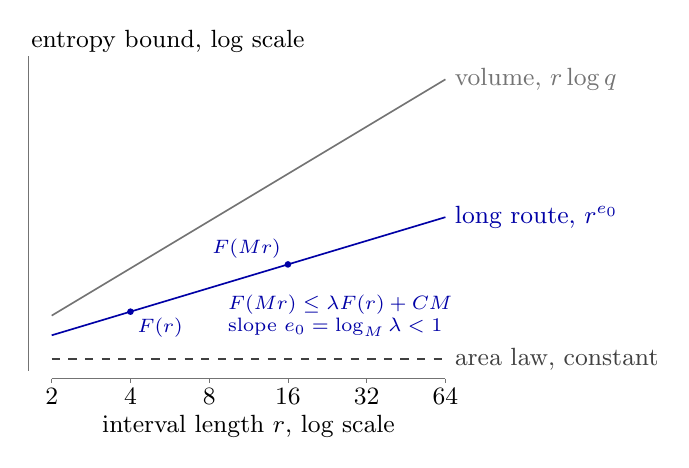
\begin{tikzpicture}[x=1cm, y=1cm, line width=0.3pt,
    lab/.style={font=\small, inner sep=1pt},
    name/.style={font=\scriptsize, text=black!55, inner sep=1pt},
    bound/.style={line width=0.6pt}]
  \def\dx{1.0}\def\dy{0.6}
  \def\xmax{5.0}\def\ymax{4.1}
  \draw[black!55] (0, 0) -- (\xmax, 0);
  \draw[black!55] (-0.3, 0.1) -- (-0.3, \ymax);
  \foreach \k/\r in {0/2, 1/4, 2/8, 3/16, 4/32, 5/64} {
    \draw[black!55] (\k*\dx, 0) -- (\k*\dx, -0.06);
    \node[lab, anchor=north] at (\k*\dx, -0.08) {\(\r\)};
  }
  \node[lab, anchor=north] at (2.5*\dx, -0.42) {interval length \(r\), log scale};
  \node[lab, anchor=south west] at (-0.3, \ymax) {entropy bound, log scale};
  \draw[bound, black!55] (0, 0.8) -- (5*\dx, {0.8 + 5*\dy});
  \node[lab, anchor=west, text=black!55] at (5*\dx + 0.08, {0.8 + 5*\dy}) {volume, \(r\log q\)};
  \draw[bound, blue!65!black] (0, 0.55) -- (5*\dx, {0.55 + 2.5*\dy});
  \node[lab, anchor=west, text=blue!65!black] at (5*\dx + 0.08, {0.55 + 2.5*\dy}) {long route, \(r^{e_0}\)};
  \draw[bound, dashed, black!75] (0, 0.25) -- (5*\dx, 0.25);
  \node[lab, anchor=west, text=black!75] at (5*\dx + 0.08, 0.25) {area law, constant};
  \fill[blue!65!black] (1*\dx, {0.55 + 0.5*\dy}) circle (1.2pt);
  \fill[blue!65!black] (3*\dx, {0.55 + 1.5*\dy}) circle (1.2pt);
  \node[name, anchor=north west, text=blue!65!black] at (1*\dx + 0.05, {0.55 + 0.5*\dy - 0.04}) {\(F(r)\)};
  \node[name, anchor=south east, text=blue!65!black] at (3*\dx - 0.05, {0.55 + 1.5*\dy + 0.04}) {\(F(Mr)\)};
  \node[name, anchor=north west, align=left, text=blue!65!black] at (2.2*\dx, 1.1)
    {\(F(Mr)\le\lambda F(r)+CM\)\\ slope \(e_0=\log_M\lambda<1\)};
\end{tikzpicture}

\end{adjustbox}
\caption{Entropy bounds for an interval of length $r$ on log–log axes (drawn with $M=4$): the volume bound $r\log q$, parallel to the diameter $r$, has slope one; the long route gives slope $e_0<1$; the area law is the constant line reached directly in the previous stage.}\label{fig:recursion}
\end{figure}

\begin{figure*}[t]
\centering
\begin{adjustbox}{max width=\linewidth}
\begin{tenkz}[lattice={1x16}, frame=plane, physical=up, bonds=none]
  \tn{} & \tn{} & \tn{} & \tn{} & \tn{} & \tn{} & \tn{} & \tn{} & \tn{} & \tn{} & \tn{} & \tn{} & \tn{} & \tn{} & \tn{} & \tn{}
  \tnmark[form=enclosure, species=selected, label pos=s]{(1,7) .. (1,10)}{$X$}
  \tnmark[form=enclosure, species=collar, label pos=n]{(1,4) .. (1,13)}{$N_{2r}(X)$}
  \tnmark[form=enclosure, species=complement, label pos=s]{(1,1) .. (1,2)}{$J$}
  \tnmark[form=enclosure, species=complement, label pos=s]{(1,15) .. (1,16)}{$J$}
\end{tenkz}

\end{adjustbox}
\caption{Amplification on the chain: the interval $X$ of length $n$, its graph neighbourhood $N_{2r}(X)$ with $r=O(n^{e_0/\alpha})=o(n)$, on which the local unitary of the amplification argument acts, and the far set $J$ it never touches, so that $I(X:J)\le n^{-M}$.}\label{fig:chain-amplify}
\end{figure*}

\begin{figure*}[t]
\centering
\begin{adjustbox}{max width=\linewidth}
\begin{tenkz}[lattice={1x16}, frame=plane, physical=up, bonds=none]
  \tn{} & \tn{} & \tn{} & \tn{} & \tn{} & \tn{} & \tn{} & \tn{} & \tn{} & \tn{} & \tn{} & \tn{} & \tn{} & \tn{} & \tn{} & \tn{}
  \tnmark[form=enclosure, species=complement, label pos=s]{(1,1) .. (1,4)}{$B$}
  \tnmark[form=enclosure, species=collar, label pos=n]{(1,5) .. (1,6)}{$D$}
  \tnmark[form=enclosure, species=selected, label pos=s]{(1,7) .. (1,7)}{$X_1$}
  \tnmark[form=enclosure, species=secondary, label pos=n]{(1,8) .. (1,9)}{$X_2$}
  \tnmark[form=enclosure, species=selected, label pos=s]{(1,10) .. (1,13)}{$X_3$}
  \tnmark[form=enclosure, species=secondary, label pos=n]{(1,14) .. (1,16)}{$X_4$}
\end{tenkz}

\end{adjustbox}
\caption{Two families on a half-line: beyond the cut and the removed sites $D$, the dyadic intervals $X_i=[2^i,2^{i+1})$ of lengths $2,4,8,\dots$ with alternating family labels, continuing to the end of the chain. Each is separated from $B$ and from all earlier same-family intervals by the previous interval, of half its length.}\label{fig:chain-families}
\end{figure*}
